%!TEX root = TIWSNE_Mini_project_main.tex
\section{Program Flow}
The program deployed on the sender mote and the receiver mote is identical, except for their note id. This is possible, since a state machine is implemented. The main idea is pretty simple. The state machine have eight states, and is controlled with the button on the mote. The LED's on the mote is used to display the current state.


The eight states reflects all the needed functionality in both the sender and receiver:
\begin{itemize}
\item Idle
\item Receiving from PC
\item Sending uncompressed to mote
\item Sending compressed to mote
\item Receiving uncompressed from mote
\item Receiving compressed from mote
\item Sending uncompressed to PC
\item Sending compressed to PC
\end{itemize}

A simplified sequence diagram of the boot sequence and a key press is shown in Figure \ref{fig:BootAndState}. On boot, the used flash areas are erased, and the key is enabled. After boot, the idle state is entered. When the key is pressed the state is changed and everything needed is initialized and the radio is turn on or off, depending on the state. Finally a task is posted to start the transmissions.

\begin{figure}[H]
\centering
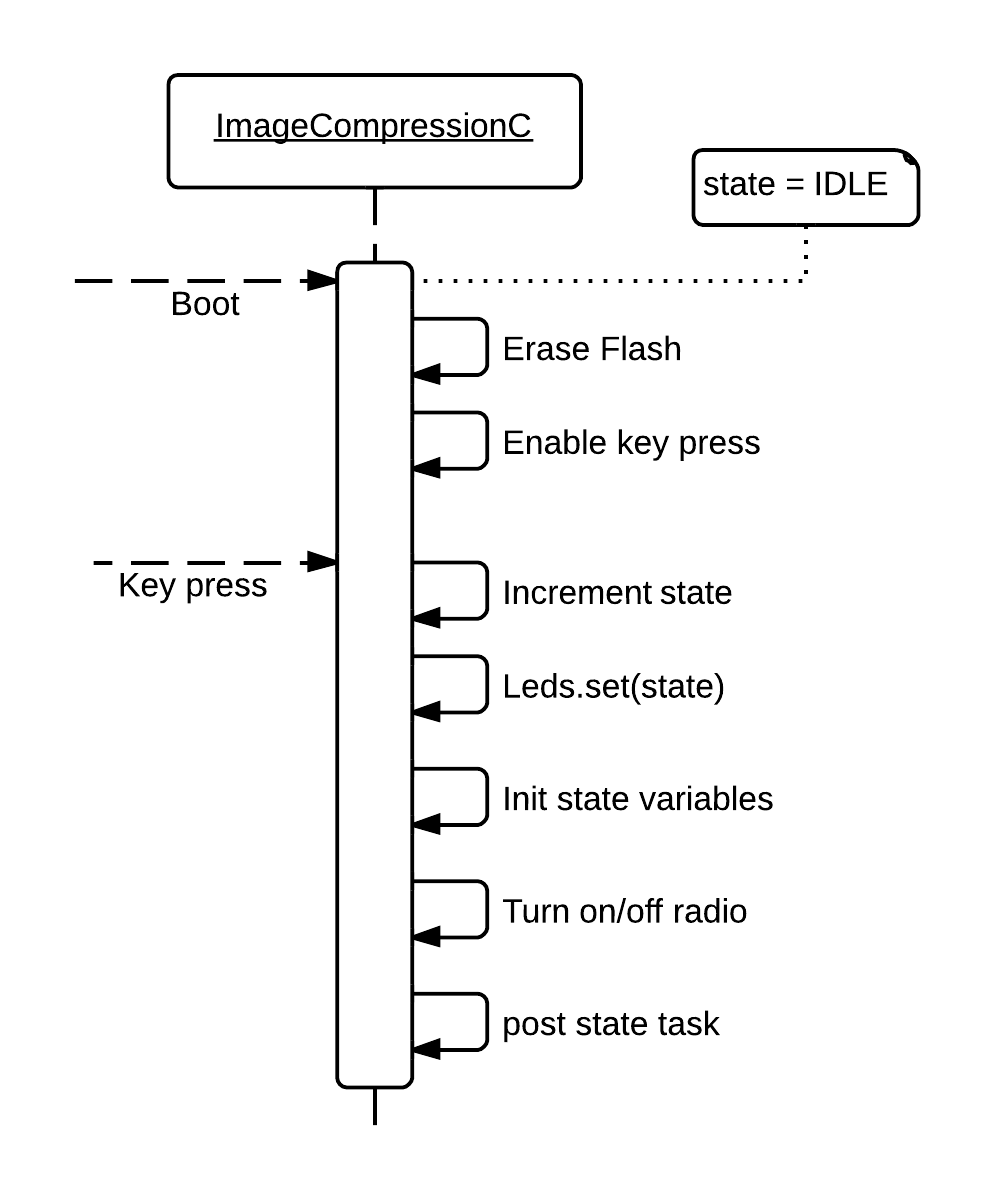
\includegraphics[width=0.5\linewidth]{BootAndStateSeq}
\caption{Simplified boot and state change sequence diagram}
\label{fig:BootAndState}
\end{figure}

In Figure \ref{fig:SendReceiveSeq} a simplified sequence diagram for the \emph{Sending compressed to mote} and \emph{Receiving compressed from mote} states are shown. Each task is initially posted when changing state and executed by the TinyOS. When sending, data is read from the flash, compressed and send. After sending, a timer is started, to be able to retransmit in case no acknowledgment is received. When the ACK is received, the task post itself again. This sequence continues until all packets have been sent, or the state is changed.

The receiving state is quite similar, it waits until it receives a packet, then decompress it and store it in the flash, and sends an ACK back to the sender.


\begin{figure}[H]
\centering
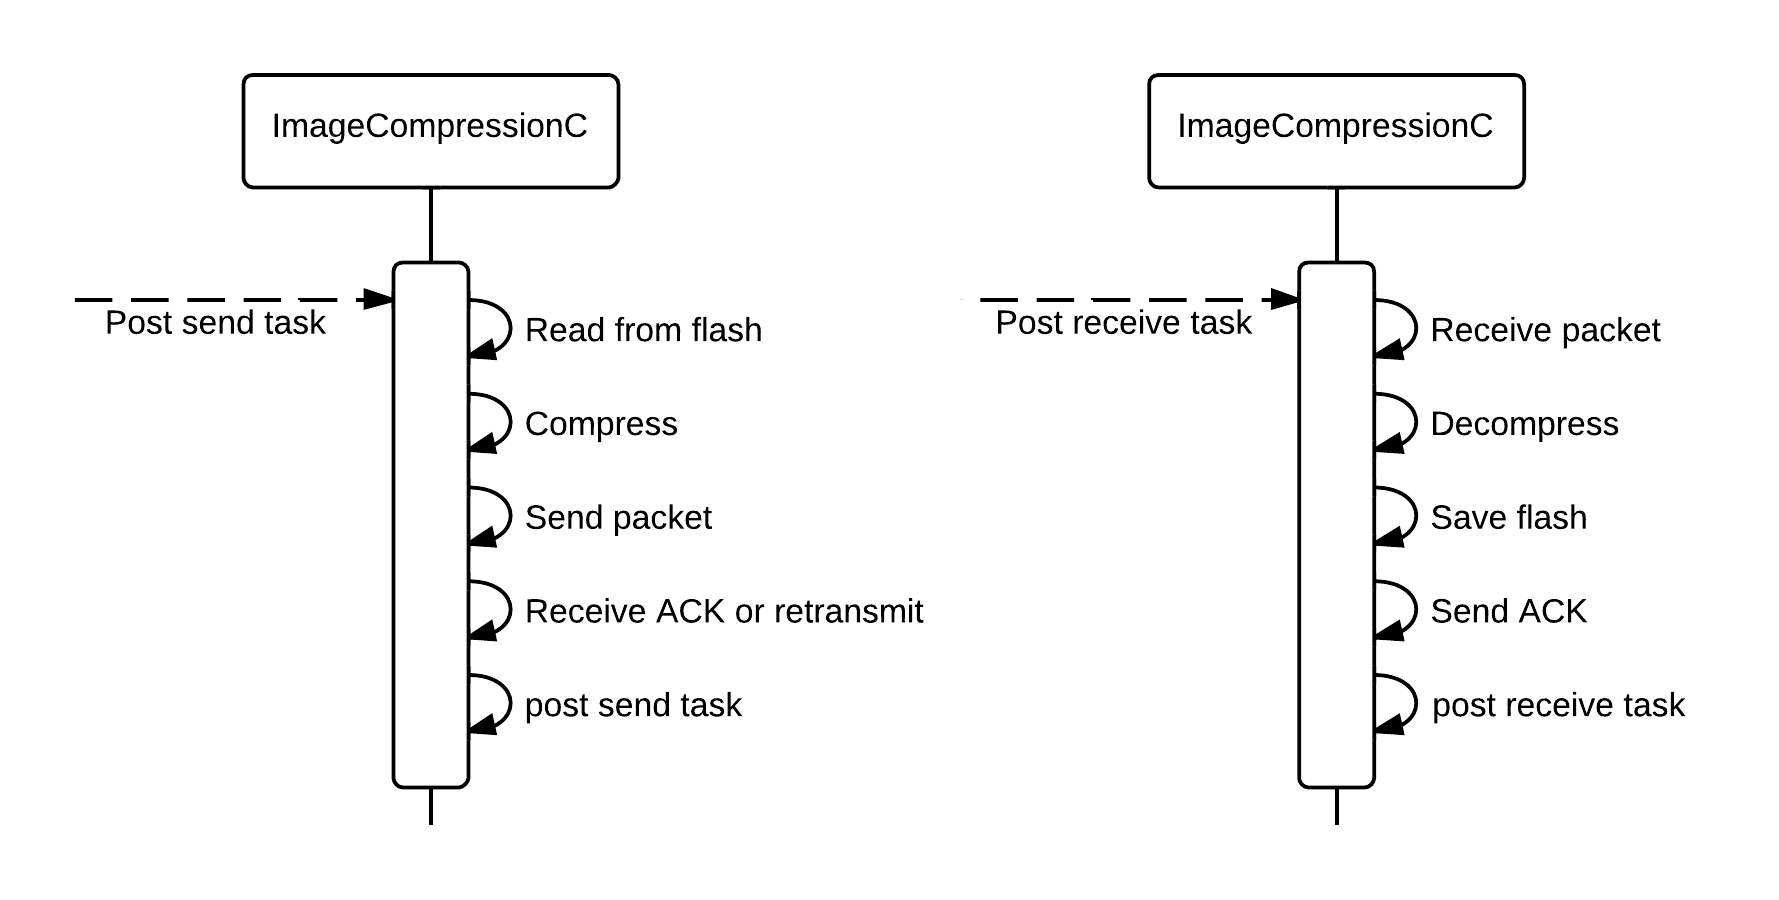
\includegraphics[width=0.9\linewidth]{SendSeq}
\caption{Simplified program flow for wireless transmission.}
\label{fig:SendReceiveSeq}
\end{figure}

The program flow for sending and receiving uncompressed packets, is exactly similar, except that the compression and decompression is removed.

Serial program flow?

Improvements in discussion